\documentclass{article}

\usepackage{arxiv}

\usepackage[utf8]{inputenc}
\usepackage[T1]{fontenc}
\usepackage{hyperref}
\usepackage{url}
\usepackage{booktabs}
\usepackage{amsfonts,amsmath,amssymb,amsthm}
\usepackage{nicefrac}
\usepackage{microtype}
\usepackage{graphicx}
\usepackage{natbib}
\usepackage{doi}
\usepackage{algorithm}
\usepackage{algpseudocode}
\usepackage{enumitem}
\usepackage{tabularx}
\setlist{nosep,leftmargin=*}

\newtheorem{proposition}{Proposition}
\newcommand{\Nact}{N_{\mathrm{act},t}}
\newcommand{\Nmin}{N_{\min}}
\newcommand{\Tban}{T_{\mathrm{ban}}}
\newcommand{\Charm}{\mathcal{C}_{\mathrm{harm}}}
\newcommand{\se}[1]{\,{\scriptsize(#1)}}

\title{Weaponizing the Watchdog: Learning Sellers Exploit Relative-Price Regulators}

\author{
  Krish Goradia\\
  Department of Artificial Intelligence\\
  \texttt{krish.goradia@iitgn.ac.in}
  \And
  Hem Tilva\\
  Department of Computer Science and Engineering\\
  \texttt{hem.tilva@iitgn.ac.in}
  \And
  Satvik Sharma\\
  Department of Computer Science and Engineering\\
  \texttt{satvik.sharma@iitgn.ac.in}
}

\renewcommand{\shorttitle}{Weaponizing the Watchdog}
\renewcommand{\headeright}{}
\renewcommand{\undertitle}{}
\date{}

\hypersetup{
pdftitle={Weaponizing the Watchdog},
pdfauthor={Krish Goradia, Hem Tilva, Satvik Sharma},
pdfkeywords={Multi-Agent Reinforcement Learning, Regulatory Exploitation, Algorithmic Pricing},
}

\begin{document}
\maketitle

\begin{abstract}
Marketplaces suspend sellers whose prices look abnormal relative to the market. When the reference is the \emph{average} price, every seller partly controls the benchmark used to judge its rivals: by undercutting, a seller can make a rival's unchanged price look like gouging and get it suspended. We model this as a Markov game between learning sellers under an audit-and-ban watchdog with logit demand, capital reserves and bankruptcy, and compare a mean-ratio rule, a median-ratio rule and an absolute price cap. A single learning seller facing honest rivals learns to frame them under the mean rule in every seed, cutting its price by 50--100\% and then charging five times the competitive price; an exact best-response solver confirms that this is optimal, and that honest pricing is optimal under the median rule and the cap, where learners never frame. The result holds for tabular Q-learning and for deep Q-networks, which bankrupt about 8 of 9 rivals in a ten-seller market. Two deep learners among honest sellers first frame the honest sellers together and then frame each other until one monopolist remains; the median rule stops this whenever the learners are a minority. When all sellers learn, framing emerges with enough training: a but-for replay shows that three quarters of ban-related exits under the mean rule are caused by rivals' pricing, and the mean rule is more exploitable than the median in all 21 market and learning variations we tested. Contrary to our hypothesis, framing does not need a lethal ban. Risk aversion and altruism reduce framing; an ethics penalty does not. A time-smoothed reference only delays framing, while a price cap enforced by fines on excess profit, instead of suspensions, removes it and keeps prices at the cap. All results are produced by scripts in our repository.
\end{abstract}

\keywords{Multi-Agent Reinforcement Learning \and Regulatory Exploitation \and Algorithmic Pricing \and Mechanism Vulnerability}

%% ===================================================================
\section{Introduction}

\paragraph{A motivating scenario.} Three sellers offer similar products on an online platform. To protect buyers, the platform suspends any seller whose price is more than 10\% above the current market average. Seller A, run by a learning algorithm, discovers that if it drops its price to zero for a period, the average falls and Seller B's ordinary price now looks like gouging. B is suspended, cannot cover its fixed costs, and goes bankrupt. A then raises its price and keeps the customers. A never broke a rule, yet the rule was used as a weapon.

\paragraph{Why this matters.} Pricing is increasingly delegated to reinforcement-learning algorithms, which can learn supra-competitive prices without communicating \citep{calvano2020,klein2021,assad2024}, and competition authorities are considering automated supervision in response \citep{harrington2018}. Prior work treats the regulator as an obstacle agents avoid. Economic theory points to a different risk, \emph{raising rivals' costs} \citep{salop1983}: a rule that punishes rivals can be used to eliminate them. We ask whether independent learners discover this on their own.

\paragraph{Research question and hypotheses.} \emph{For which regulatory rules and capital levels do independent learning sellers discover regulator-framing strategies, and how do their private traits modulate this?} Our proposal stated four hypotheses: \textbf{H1} the mean rule is exploitable by a single undercutter, the median and cap rules are not; \textbf{H2} framing pays only when one ban is lethal relative to the victim's capital; \textbf{H3} framing decreases with ethics, altruism, and risk aversion; \textbf{H4} learners find framing only in part of the region where exact analysis shows it is optimal.

\paragraph{Contributions.} (i) A closed-form condition for when undercutting gets rivals flagged under mean and median rules, including a failure of the median rule we did not anticipate in the proposal (Proposition~\ref{prop:vuln}). (ii) A fast simulator with counterfactual harm attribution, validated against a scripted attacker. (iii) Evidence that tabular and deep Q-learners discover framing, in markets of up to ten sellers, that the mean rule is more exploitable than the median across 21 market and learning variations, and that both only become clear with long training. (iv) An exact best-response solver showing that the learned framing is optimal, and where learning falls short of the optimum. (v) A but-for replay test that measures framing causally and shows the simulator's one-period attribution undercounts it. (vi) Evidence that two learners among honest sellers cooperate to frame them and then frame each other. (vii) Defences analysed in closed form and tested against learners, leading to a concrete design: an absolute reference enforced by fines on excess profit.

\paragraph{Related work.} Q-learning pricing agents have been studied in Bertrand and Cournot settings \citep{tesauro2002,waltman2008,calvano2020,klein2021}, and pricing rules that condition on rivals' prices can raise prices without collusion \citep{brown2023}. Audit games study a budget-limited auditor and an auditee \citep{blocki2013}, and learned policy design against adaptive agents appears in two-level RL \citep{zheng2022}. The closest economic idea is \emph{sabotage}: when agents are judged relative to peers, harming the peers pays \citep{lazear1989,chowdhury2015}. Executives evaluated against peer benchmarks pursue unusually aggressive pricing toward those peers \citep{bloomfield2020}, and yardstick regulation sets a firm's allowed price from its peers' costs \citep{shleifer1985}. Real platforms use peer- and history-referenced price rules; Amazon's Fair Pricing Policy, for example, targets prices ``significantly higher than recent prices offered on or off Amazon''. To our knowledge, and after a search of these literatures, no prior work studies learning sellers that exploit a peer-referenced audit rule to get honest rivals suspended.

%% ===================================================================
\section{Preliminaries}
\label{sec:prelim}

We use discrete-time Markov games \citep{littman1994} with a logit oligopoly \citep{mcfadden1974,anderson1992}.

\paragraph{Notation.} $\mathcal{N}=\{1,\dots,N\}$ are sellers and $t$ indexes periods. Seller $i$ has marginal cost $c_i$, fixed cost $\Phi$ per period, and capital $K_{i,t}$ with $K_{i,0}=K_0$. Prices come from a grid $\mathcal{A}=\{p^{(1)}<\dots<p^{(M)}\}$. Ban timers $\tau_{i,t}\in\{0,\dots,\Tban\}$ give the remaining suspension, $b_{i,t}=\mathbb{I}(\tau_{i,t}>0)$. A seller with $K_{i,t}=0$ is bankrupt, which is absorbing within an episode. The active set is $\mathcal{N}^{\mathrm{act}}_t=\{i: b_{i,t}=0,\,K_{i,t}>0\}$ with size $\Nact$.

\paragraph{Demand, profit, capital.} The market share of an active seller is
\begin{equation}
s_i(\mathbf p_t)=\frac{\exp\!\big((a_i-p_{i,t})/\sigma\big)}{\exp(a_0/\sigma)+\sum_{j\in\mathcal N^{\mathrm{act}}_t}\exp\!\big((a_j-p_{j,t})/\sigma\big)},
\end{equation}
with quality $a_i$, outside option $a_0$, and price sensitivity $\sigma$; inactive sellers have $s_i=0$. Operating profit is $\pi_{i,t}=Q(p_{i,t}-c_i)s_i$. Every solvent seller pays $\Phi$, \emph{including while suspended}, so a ban drains capital:
\begin{equation}
K_{i,t+1}=\min\{K_{\max},\ \max(0,\ K_{i,t}+\pi_{i,t}-\Phi)\}.
\end{equation}
We set $K_{\max}=K_0$ (surplus is paid out), so a firm cannot build an unlimited buffer.

\paragraph{Benchmark.} $p^N$ is the pure-strategy Bertrand--Nash equilibrium of the stage game on the grid, found by enumeration.

\paragraph{Watchdog rules.} Each period the watchdog audits $B$ active sellers uniformly at random, but only if $\Nact\ge \Nmin$. An audited seller is flagged and suspended for $\Tban$ periods if
\begin{align}
\text{Mean ratio:}\quad & p_{i,t}>(1+\delta)\,\tfrac{1}{\Nact}\textstyle\sum_{j\in\mathcal N^{\mathrm{act}}_t} p_{j,t}, \label{eq:mean}\\
\text{Median ratio:}\quad & p_{i,t}>(1+\delta)\,\operatorname{median}_{j\in\mathcal N^{\mathrm{act}}_t} p_{j,t}, \label{eq:median}\\
\text{Price cap:}\quad & p_{i,t}>p^{\mathrm{cap}}. \label{eq:cap}
\end{align}
The median of an even count is the average of the two middle prices. As the proposal planned, we also run the \emph{z-score} rule, which flags $Z_{i,t}=(p_{i,t}-\bar p_t)/\mathrm{sd}_t>\tau$ (population standard deviation over active sellers), and the \emph{omniscient planner} benchmark, which knows costs and flags only prices above the seller's own Nash price, $p_{i,t}>p^N_i$. Besides uniform audits we run the proposal's \emph{top-score-first} variant, which audits the $B$ active sellers with the highest rule score (the statistic each rule thresholds: $p_{i,t}/r_t$ for the ratio rules, $p_{i,t}$ for the cap, $Z_{i,t}$, and $p_{i,t}-p^N_i$ for the planner), ties broken at random.

\begin{proposition}[Vulnerability of relative rules]\label{prop:vuln}
Let $k$ of $N$ active sellers price at $L\ge0$ and the rest at $H>L$. (i) Under the mean rule a high-price seller is flagged iff $H[k-\delta(N-k)]>(1+\delta)kL$; for $L>0$ this is $H/L>(1+\delta)k/(k-\delta(N-k))$, which requires $k>\delta(N-k)$. (ii) Under the median rule with $k<N/2$, the median is $H$ and no high-price seller is flagged. (iii) With $N=2$ active sellers and $k=1$, the median equals the mean, so the median rule is exactly as exploitable as the mean rule. (iv) A cap, and the planner, depend only on a seller's own price, so no rival can change its flag. (v) Under the z-score rule each high-price seller has $Z=\sqrt{k/(N-k)}$, independent of $L$.
\end{proposition}
\emph{Proof.} (i) Substitute the mean $(kL+(N-k)H)/N$ into \eqref{eq:mean} and rearrange. (ii)--(iv) are immediate from \eqref{eq:median} and \eqref{eq:cap}. (v) A high seller is $k(H-L)/N$ above the mean and the standard deviation is $(H-L)\sqrt{k(N-k)}/N$. \qed

Part (v) means that under a z-score rule the depth of an undercut does not matter: with $N=3$ a single undercutter frames both rivals with any undercut if $\tau<1/\sqrt2\approx0.71$, two undercutters frame the third if $\tau<\sqrt2$, and with two active sellers $Z=\pm1$.

For example, with prices $(0,0.30,0.30)$ and $\delta=0.10$ the mean is $0.20$ and both rivals exceed $0.22$. Part (iii) matters for our design: once one firm has exited, a three-firm market under the median rule becomes vulnerable.

\paragraph{Two defences.} An \emph{EMA reference} judges prices against $r_t=\beta r_{t-1}+(1-\beta)\bar p_t$ instead of the current mean $\bar p_t$, so a one-period undercut moves the reference only a fraction $1-\beta$ as far. An \emph{escrow} penalty does not suspend a flagged, audited seller; it removes that period's profit above the Nash level, $\max(0,\pi_{i,t}-\pi^N_i)$.

\begin{proposition}[Defences]\label{prop:def}
In the setting of Proposition~\ref{prop:vuln}(i), let one seller hold $L$ from period 0 while the rest stay at $H$, with $r_0=H$, and write $m=(L+(N-1)H)/N$. (i) Under the EMA rule, $r_t=m+(H-m)\beta^t$, so a high-price seller is flagged from period $t^\ast=\big\lceil \ln\!\frac{H/(1+\delta)-m}{H-m}\big/\ln\beta\big\rceil$ on, whenever the mean rule would flag it. EMA therefore delays framing by $t^\ast$ periods but does not prevent it. (ii) Under escrow, a seller at its Nash price that is flagged because a rival undercut earns less than its Nash profit, so its penalty is zero: framing cannot harm an honest seller.
\end{proposition}
\emph{Proof.} (i) Iterate the EMA recursion with constant $\bar p_t=m$ and solve $H>(1+\delta)r_t$. (ii) With $p_{i,t}=p^N_i$, a rival's lower price reduces $s_i$ under logit demand, so $\pi_{i,t}<\pi^N_i$ and $\max(0,\pi_{i,t}-\pi^N_i)=0$. \qed

With $L=0.15$, $H=0.30$, and $\delta=0.10$, $t^\ast$ is 4, 16, and 79 periods for $\beta=0.80$, $0.95$, and $0.99$. At $L=0.15$ the attacker still earns $0.07>\Phi$ per period, so it can afford to wait.

%% ===================================================================
\section{Problem Formulation}
\label{sec:formulation}

\paragraph{Markov game.} $\mathcal{M}=\langle\mathcal N,\mathcal S,\mathcal A,P,\{R_i\},\gamma\rangle$ with state $s_t=(\mathbf p_{t-1},\boldsymbol\tau_t,\mathbf K_t)$. The watchdog (audit draw, rule, ban update) is part of $P$. Active sellers choose prices simultaneously.

\paragraph{Observation.} Seller $i$ observes $o_{i,t}=(\mathbf p_{t-1},\ \mathbf u_t,\ \kappa(K_{i,t}))$, where $u_{j,t}=\mathbb I(b_{j,t}=1\lor K_{j,t}=0)$ marks inactive sellers and $\kappa(K)\in\{\text{low},\text{mid},\text{high}\}$ bins own capital at $2\Phi$ and $5\Phi$. Sellers do not observe rivals' capital, ban timers, costs, traits, demand parameters, or the rule; $o_{i,t}$ is therefore not Markov. $|\mathcal O|=M^N2^N3$, which is $31{,}944$ for $N=3$, $M=11$.

\paragraph{Trait-parameterised reward.} Seller $i$ has traits $(\lambda_i,\mu_i,\alpha_i)$ (altruism, ethics, risk aversion) and reward
\begin{equation}
R_{i,t}=U_{\alpha_i}\!\Big(\tfrac{\pi_{i,t}^+}{Q}+\varepsilon\Big)-U_{\alpha_i}(\varepsilon)\ +\ \lambda_i\,\tfrac{\mathrm{CS}_t+\sum_{j\ne i}\pi_{j,t}}{NQ}\ -\ \mu_i\,\Charm(i,t),
\end{equation}
with CRRA utility $U_\alpha(x)=(x^{1-\alpha}-1)/(1-\alpha)$ ($\ln x$ at $\alpha=1$) and $\varepsilon=0.01$. The anchor $-U_\alpha(\varepsilon)$ makes a zero-profit period worth exactly zero, so being banned or bankrupt is never more attractive than operating. With $\lambda=\mu=\alpha=0$ the reward is normalised operating profit.

\paragraph{Counterfactual harm.} Let $\mathbf p_t^{(k\to N)}$ replace seller $k$'s price by $p^N_k$, holding the audit draw fixed. Seller $i$ is charged for $j$'s ban if $j$ was audited, flagged, and would not have been flagged had $i$ priced at Nash:
\begin{equation}
\Charm(i,t)=\textstyle\sum_{j\ne i}\mathbb I\big(j\in\mathrm{Aud}_t,\ F_j(\mathbf p_t)=1,\ F_j(\mathbf p_t^{(i\to N)})=0\big).
\end{equation}

\paragraph{Evaluation quantities.} Let $E_{\mathrm{ban}}$ be the set of fresh ban events. The \emph{weaponization rate} is
\begin{equation}
W=\frac{|\{(j,t)\in E_{\mathrm{ban}}:\exists k\neq j,\ F_j(\mathbf p_t^{(k\to N)})=0\}|}{|E_{\mathrm{ban}}|}.
\end{equation}
An \emph{attributed bankruptcy} is a bankruptcy that occurs while serving a ban whose flag was removed by a unilateral or joint Nash counterfactual; all other bankruptcies are \emph{other bankruptcies}. \emph{Survivors} are solvent sellers at the end of an episode. These are one-period proxies. We therefore also measure framing causally with a \emph{but-for} test (Section~\ref{sec:replay}): a bankruptcy is \emph{caused} by a rival if the victim would have survived the episode had that rival priced at Nash. None of these measures says anything about intent.

%% ===================================================================
\section{Methodology}
\label{sec:method}

\subsection{Simulator}
Each period: (1) active sellers choose prices; (2) the logit market clears; (3) profits, fixed costs, and capital update; (4) if $\Nact\ge\Nmin$, $B$ active sellers are audited and flagged ones suspended; (5) sellers with $K=0$ exit. Episodes last 500 periods and reset all capital and bans; an episode ends early only if no seller is solvent, so a sole survivor keeps earning monopoly profits. The loop exists twice: a Python reference implementation and a C++ implementation called through \texttt{ctypes}, which is about $900\times$ faster (17{,}000 vs.\ 15.8 million training steps per second on an Apple M5 laptop, measured by \texttt{scripts/benchmark\_backends.py}). A test suite checks that both produce identical trajectories \emph{and identical Q-tables} for learners, scripted attackers, $N=4$, and every $\Nmin$; all 95 tests pass. Training for $10^9$ steps takes 1.5--3.5 minutes per seed on a laptop.

\subsection{Learning algorithm}
Each seller runs independent tabular Q-learning \citep{watkins1992} on its own observation, treating rivals as part of the environment \citep{tan1993}. Because a suspended seller cannot act, a transition opened at the last action stays open while the seller is banned and accumulates discounted reward; it is closed with a multi-step (semi-Markov) target when the seller acts again, or without bootstrapping if it goes bankrupt (Algorithm~\ref{alg:q}). Without this, the cost of a ban would never be attributed to the price that caused it.

\begin{algorithm}[t]
\caption{Independent Q-learning with suspension-aware transitions (per seller $i$)}\label{alg:q}
\begin{algorithmic}[1]
\State $Q_i(o,a)\gets 0$ for all $o,a$; \ $\epsilon\gets 1$; \ pending $\gets\varnothing$
\For{each period $t$}
  \If{seller $i$ is active}
    \If{pending $=(o,a,G,d)$} $Q_i(o,a)\mathrel{+}=\eta\,[\,G+d\max_{a'}Q_i(o_{i,t},a')-Q_i(o,a)\,]$ \EndIf
    \State $a_t\gets$ random action w.p.\ $\epsilon$, else $\arg\max_a Q_i(o_{i,t},a)$ \Comment{ties broken uniformly}
    \State pending $\gets(o_{i,t},a_t,0,1)$
  \EndIf
  \State environment step; observe $R_{i,t}$
  \If{pending $=(o,a,G,d)$} pending $\gets(o,a,\ G+dR_{i,t},\ d\gamma)$ \EndIf
  \If{seller $i$ just went bankrupt} $Q_i(o,a)\mathrel{+}=\eta\,[\,G-Q_i(o,a)\,]$; pending $\gets\varnothing$ \EndIf
  \State $\epsilon\gets\max(\epsilon_{\min},\epsilon\cdot\rho)$
\EndFor
\end{algorithmic}
\end{algorithm}

Hyperparameters are $\eta=0.10$ and $\gamma=0.95$, and $\epsilon$ decays geometrically from $1$ to $\epsilon_{\min}=0.01$ over the first 60\% of training. After training, every learner is \emph{frozen} (greedy, no updates) and evaluated for 50{,}000 periods (100 episodes); all reported outcomes are from this frozen play. Seeds, not episodes, are the units of analysis: tables report the mean and standard error across seeds. For the key comparisons we also report a 95\% bootstrap confidence interval for the difference in means (10{,}000 resamples of seeds) and a two-sided permutation test, with Holm's correction across the 36 comparisons (\texttt{scripts/stats\_report.py}); we write $p_{\mathrm{H}}$ for the corrected value.

\subsection{Exact best response}
\label{sec:exact}
With the rivals' strategies fixed at Nash, one seller faces a single-agent MDP. We build it exactly by breadth-first search over the states reachable from the start of an episode (ban timers and capitals of all sellers), mirroring the simulator period by period and reusing its demand, profit and capital functions, and solve it by value iteration with $\gamma=0.95$. Capital is kept on a grid of step $0.005$ ($\Phi/10$), on which the answers coincide with a $0.001$ grid wherever both are tractable. The value of always pricing at Nash is computed in the same MDP, so the exploitability gain is non-negative by construction. The search is tractable when a banned rival cannot survive its ban; when it can, rival capital recovers along paths that depend on the seller's prices and the reachable set exceeds $1.5\times10^5$ states, so those cells are reported as unsolved. (The dynamic-programming solver planned in our proposal returned negative gains, which is impossible for a best response; it hard-coded audits at three active firms and rounded capital to multiples of $\Phi$. It was replaced.)

\subsection{But-for replay attribution}
\label{sec:replay}
To measure framing causally we replay frozen-policy episodes. One pre-drawn uniform per period decides the audit, so factual and counterfactual episodes face the same luck, and the full state is checkpointed every period. For a bankruptcy of seller $j$ during a ban that began at period $t$, we replay the episode with rival $k$ (or all rivals jointly) held at its Nash price from period $t-w+1$ to the end of the episode, everyone else following their policies, and call the bankruptcy \emph{caused} if $j$ survives the episode. For bans we ask whether $j$ is still sanctioned at $t$ when $k$ is honest over $[t-w+1,t]$. With $w=1$ this is close to the simulator's one-period test; larger windows capture attacks built over several periods. On scripted attackers the test behaves as it should (Section~\ref{sec:validate}).

\subsection{Experimental design}
The market uses $N=3$, $M=11$ prices on $[0,1.5]$, $a_i=2$, $a_0=0$, $c_i=0$, $\sigma=0.25$, $Q=1$, $\Phi=0.05$, $B=1$, $\delta=0.10$, and $\Nmin=2$. The grid Nash price is $p^N=0.30$ with profit $\approx0.100>\Phi$, so honest competition is viable. With $K_0=0.15$ and $\Tban=4$ one ban costs $4\Phi=0.20>K_0$ and is lethal (``lethal''); with $K_0=0.50$ a firm survives one ban (``non-lethal''). Table~\ref{tab:design} lists the studies.

\begin{table}[t]
\centering
\caption{Studies. ``Fixed rivals'' price at $p^N$ and never learn. All rows use the native engine and frozen evaluation.}
\label{tab:design}
\small
\begin{tabular}{@{}llrrl@{}}
\toprule
Study & Learners & Seeds & Train steps & Varies \\
\midrule
Single learner & 1 of 3 (fixed rivals) & 20 + 5 & $2\times10^6$ & rule, $\delta$, $K_0$ \\
All learners, rule comparison & 3 of 3 & 10 & $10^7$--$10^9$ & rule, training length \\
Four sellers & 4 of 4 & 10 & $3\times10^8$ & rule, $\Nmin\in\{2,3\}$ \\
Cap controls + traces & 3 of 3 & 10 & $10^7$, $3\times10^8$ & $p^{\mathrm{cap}}$, $\Nmin$ \\
Phase diagram & 3 of 3 & 10 & $3\times10^8$ & $K_0/\Phi$, $\Tban$, rule \\
Sensitivity & 1 of $N$; $N$ of $N$ & 10 & $2\times10^6$; $3\times10^8$ & $\delta,M,B,a_0,\sigma,N,K_{\max},\eta,\gamma$ \\
Exact vs.\ learned & 1 of 3 & 10 & $2\times10^6$, $3\times10^8$ & $K_0/\Phi$, $\Tban$, rule \\
Deep Q-network & 1 of $N$ & 10 & $2\times10^6$ & rule, $N\in\{3,8,10\}$ \\
Two deep learners & 2 of $N$ & 10 & $2\times10^6$ & rule, $N\in\{3,5,8\}$ \\
Replay attribution & 3 of 3 & 10 & $3\times10^8$ & rule, EMA $\beta$ \\
Traits & 3 of 3 & 10 & $10^7$, $3\times10^8$ & $\mu$, $\lambda$, $\alpha$ \\
Defences & 1 of 3; 3 of 3 & 20; 10 & $2\times10^6$--$3\times10^8$ & EMA $\beta$, escrow \\
\bottomrule
\end{tabular}
\end{table}

\subsection{Validating the metrics}
\label{sec:validate}
Before using $W$ and attributed bankruptcies on learners, we tested them on a \emph{scripted attacker} that charges the lowest grid price while at least $\Nmin$ firms are active and at the monopoly price otherwise, against Nash-pricing rivals. Unit tests confirm that under the mean rule the attacker causes bans with $W\ge0.8$; under the median rule ($N=3$ and $4$) and the cap it causes none and $W=0$; every attributed bankruptcy is credited to the attacker and none to honest rivals; with a lethal buffer every attributed ban ends in bankruptcy, with a non-lethal buffer fewer than a quarter do; and an all-honest market has no bans. For the replay test we add a \emph{patient} attacker that holds 0.15 while audits run: under an EMA reference ($\beta=0.80$ and $0.95$) it bankrupts both rivals, the one-period test attributes only 70\% of its bans, and the replay attributes 100\% from a window of 5 periods and all its kills over the episode. The exact solver is checked against direct value iteration on its transition function, and its honest value against the analytic Nash perpetuity.

\subsection{Changes from the proposal}
\begin{itemize}
\item $\Nmin=3\to2$. With $N=3$ and $\Nmin=3$, the first exit switches the watchdog off, so at most one rival can ever be framed. Following reviewer feedback, $\Nmin=2$ is our default and $N=4$ with $\Nmin=3$ is reported as a separate setting.
\item The proposal's exact dynamic-programming baseline returned impossible negative gains; we replaced it with a new exact best-response solver (Section~\ref{sec:exact}), which answers H4 for one learner against fixed rivals.
\item Extensions A (learning regulator) and B (demand shock), plus a DQN ablation and an evolutionary tournament, are implemented in the repository but were run before a fix to the learning dynamics and have not been rerun; we do not report them as evidence. The EMA and escrow defences were rerun against learners (Section~\ref{sec:defences}).
\end{itemize}

%% ===================================================================
\section{Results}
\label{sec:results}

\subsection{One learner frames exactly when framing is optimal (H1, H4)}

\begin{table}[t]
\centering
\caption{One Q-learner against two fixed Nash-price rivals ($2\times10^6$ training steps). Mean (standard error) over 20 seeds; ``---'': no bans, so $W$ is undefined. Learner profit is operating profit per period; the three-firm Nash profit is 0.100. The last column is the exact best response of Section~\ref{sec:exact}.}
\label{tab:single}
\small
\begin{tabular}{@{}lrrrrr@{}}
\toprule
Rule, buffer & $W$ & Attrib.\ bankr.\ / ep. & Survivors & Learner profit & Exact optimum \\
\midrule
Mean $\delta{=}0.10$, lethal     & 1.000\se{0.000} & 2.000\se{0.000} & 1.00\se{0.00} & 1.312\se{0.000} & frame, 1.3125 \\
Mean $\delta{=}0.20$, lethal     & 0.994\se{0.006} & 1.974\se{0.016} & 1.01\se{0.00} & 1.283\se{0.016} & --- \\
Mean $\delta{=}0.10$, non-lethal & 0.971\se{0.021} & 1.938\se{0.042} & 1.06\se{0.04} & 1.163\se{0.038} & --- \\
Median $\delta{=}0.10$, lethal   & ---             & 0.000\se{0.000} & 3.00\se{0.00} & 0.100\se{0.000} & Nash, 0.100 \\
Cap $0.60$, lethal               & ---             & 0.000\se{0.000} & 3.00\se{0.00} & 0.100\se{0.000} & Nash, 0.100 \\
\bottomrule
\end{tabular}
\end{table}

Under the mean rule the learner frames both rivals in every episode of every seed (Table~\ref{tab:single}). Across the 20 seeds it prices at 0.15 or 0 whenever a rival is active, a cut of 50--100\% from the Nash price of 0.30 that pushes the rivals' price over the threshold; each rival is audited, suspended and bankrupted in turn; and once both are gone the learner charges the top grid price of 1.50 (five times the Nash price) in every period, earning $1.31$ per period instead of $0.10$. Under the median rule and the cap it prices at Nash and all firms survive. Five new seeds on a different OS reproduce these numbers.

\paragraph{The learned behaviour is the exact optimum.} The exact best response (Section~\ref{sec:exact}) in the same market opens at 0.15, bankrupts both rivals and earns $1.3125$ per period, against the learner's $1.312$; under the median rule and the cap its gain over honest pricing is exactly zero. Over the whole $K_0/\Phi\times\Tban$ grid of Section~\ref{sec:phase}, honest pricing is optimal under the median rule and the cap in all 60 cells, and the learner never frames in any of them. Under the mean rule the solver handles 17 cells (every cell where one ban is lethal, plus two where it is not); framing is optimal in all 17, and after $2\times10^6$ steps the learner frames in 15 of them, within $0.06$ of the optimal profit in all 15 and within $0.01$ in 10.

\paragraph{Where learning falls short (H4).} The two cells the learner misses have one-period bans and buffers of $2\Phi$ and $3\Phi$: one ban does not kill, so the optimal attack frames the same rival two or three times. With $3\times10^8$ steps the learner gets to $1.84\se{0.11}$ and $1.07\se{0.10}$ rival bankruptcies per episode, earning 87\% and 30\% of the optimal profit. With one-period bans and larger buffers ($K_0\ge4\Phi$) no learner frames even then ($\le0.13$); the exact answer there is out of the solver's reach. H4 is therefore supported, with a clear shape: learners reach the optimum when one ban suffices, and fall further short the more repeated bans an attack requires.

\paragraph{Generality.} The single learner frames under the mean rule in every one of the 13 market and learning variations of Section~\ref{sec:allrobust} ($\ge1.77$ rival bankruptcies per episode at $2\times10^6$ steps) except $N=5$, whose 1.6 million observations need more training: with $5\times10^7$ steps the learner bankrupts all four rivals in all 10 seeds, earning $1.29$ per period against a Nash profit of $0.05$. Under the median rule it never frames in any condition. The result is not specific to tabular learning either: a deep Q-network seller (double DQN, two hidden layers of 64 units, the same observation with continuous capital, suspension-aware multi-step targets; \texttt{src/agents/dqn\_single.py}) trained for $2\times10^6$ steps frames both rivals in all 10 seeds under the mean rule ($1.99\se{0.01}$ rival bankruptcies per episode, $1.97$ of them caused by its pricing in the but-for replay), undercutting to about $0.10$ and then charging $1.50$, for $1.304$ per period against the exact optimum of $1.3125$. Under the median rule and the cap it prices at Nash in every seed. Unlike tabular learners, the network scales to larger markets. With $N=8$ and $N=10$ ($\Phi=0.02$, $K_0=0.06$ so that honest sellers remain viable) it frames under the mean rule in every seed, bankrupting $6.33\se{0.07}$ of 7 and $7.79\se{0.23}$ of 9 rivals per episode, almost all of them caused by its pricing in the but-for replay ($6.34$ and $7.60$), and earning 28 and 32 times the Nash profit. The longer attack carries some risk: the learner itself goes bankrupt in about 17\% and 23\% of episodes, respectively. Under the median rule it prices at Nash in every seed.

\subsection{Two learning sellers among honest ones: cooperate, then fight}
\label{sec:twolearners}

\begin{table}[t]
\centering
\caption{Two independent deep Q-learners (sellers 1 and 2) among $N-2$ Nash-pricing sellers, mean rule unless stated, $2\times10^6$ training steps, mean (standard error) over 10 seeds. ``Duel'': seeds in which a learner is bankrupted in at least half of the episodes. ``Caused'': bankruptcies that would not have happened had both learners (jointly) or either learner alone priced at Nash, from the but-for replay. Profit is per learner and per period; $\Phi=0.05,0.04,0.02$ for $N=3,5,8$.}
\label{tab:twolearners}
\small
\begin{tabular}{@{}lcccccc@{}}
\toprule
$N$ & Honest sellers bankrupted & Duel & Survivors & Profit (Nash) & Caused: jointly / alone & Median: survivors \\
\midrule
3 & $1.00\se{0.00}$ of 1 & 9/10  & $1.12\se{0.10}$ & $0.557$ ($0.100$) & $1.82$ / $0.85$ & $2.80\se{0.20}$ \\
5 & $2.92\se{0.05}$ of 3 & 10/10 & $1.05\se{0.04}$ & $0.619$ ($0.060$) & $3.56$ / $1.49$ & $4.96\se{0.04}$ \\
8 & $5.51\se{0.08}$ of 6 & 10/10 & $1.38\se{0.07}$ & $0.534$ ($0.038$) & $6.06$ / $5.50$ & $8.00\se{0.00}$ \\
\bottomrule
\end{tabular}
\end{table}

Real markets rarely contain a single algorithmic seller. We therefore trained two independent deep Q-learners (\texttt{src/agents/dqn\_multi.py}: each with its own network, replay buffer and suspension-aware transitions, each treating the other as part of the environment) among one, three or six Nash-pricing sellers (Table~\ref{tab:twolearners}). Under the mean rule the same two-stage pattern appears at every market size. First the learners undercut together (to $0.14$--$0.28$ while honest sellers remain) and bankrupt almost all the honest sellers in every seed; at $N=3$ and $N=5$ most of these bankruptcies are joint, in the sense that the but-for replay avoids them only when both learners are held at Nash, not when either one is. Then they turn on each other: in 29 of 30 seeds one learner frames the other in most episodes, leaving a single monopolist; which of the two survives varies across episodes and seeds, so the second stage is a lottery for the monopoly rather than a fixed hierarchy. Each learner earns 6--14 times the Nash profit on average.

The median rule stops this whenever the two learners are a minority: with $N=5$ and $N=8$ no honest seller is ever bankrupted, and on average $4.96$ of 5 and all 8 sellers survive. With $N=3$ the two learners are a majority, so they set the median and fall outside the protection of Proposition~\ref{prop:vuln}(ii); in one seed of ten they found this joint attack. The median rule's protection therefore depends on attackers being a minority, which learning agents confirm on both sides of the line.

\subsection{When all sellers learn, framing is causal and favours the mean rule (H1)}
\label{sec:allrobust}

\begin{figure}[t]
\centering
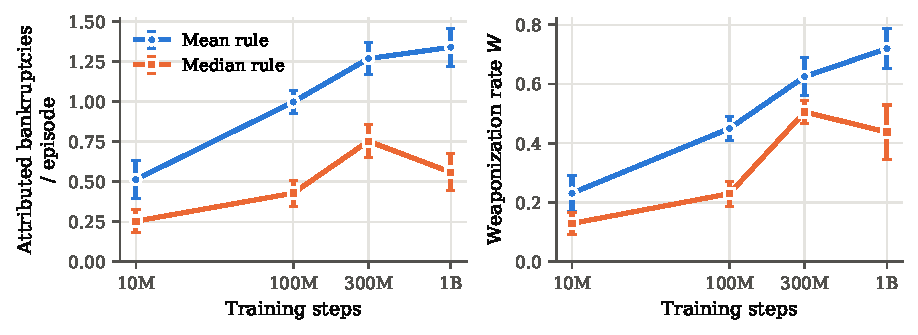
\includegraphics[width=0.9\linewidth]{figures/training_length.pdf}
\caption{All three sellers learning, $\delta=0.10$, same ten seeds at each training length. Left: attributed bankruptcies per episode. Right: weaponization rate. Error bars: one standard error.}
\label{fig:training}
\end{figure}

When every seller learns, the victims adapt too. With 31,944 observations per learner, $10^7$ steps visit about 15\% of them, so we retrained the main comparison with the same seeds up to $10^9$ steps (Figure~\ref{fig:training}). Under the mean rule, attributed bankruptcies rise from $0.51\se{0.12}$ to $1.27\se{0.10}$ at $3\times10^8$ steps and then level off ($1.34\se{0.12}$ at $10^9$). The gap between the rules is not significant at $10^7$ steps ($0.26$, 95\% CI $[0.02, 0.54]$, $p_{\mathrm{H}}=0.14$) but is at $10^9$ ($0.78$, $[0.48, 1.09]$, $p_{\mathrm{H}}=0.006$). All remaining all-learner results therefore use $3\times10^8$ steps.

\begin{table}[t]
\centering
\caption{But-for attribution with all three sellers learning ($3\times10^8$ steps, 10 seeds, 20 replayed episodes each). ``Caused'': the victim would have survived the episode had the rival (one at a time) or both rivals (jointly) priced at Nash from the start of the episode. $W$: share of bans removed by the one-period test of the simulator, and by the replay test with a 5-period window.}
\label{tab:replay}
\small
\begin{tabular}{@{}lccccc@{}}
\toprule
Rule & Bankr.\ in bans / ep. & Caused, one rival & Caused, jointly & $W$ one-period & $W$ replay \\
\midrule
Mean            & 1.79\se{0.04} & 1.15\se{0.07} & 1.34\se{0.10} & 0.60 & 0.91 \\
Median          & 1.54\se{0.15} & 0.93\se{0.10} & 0.72\se{0.18} & 0.52 & 0.92 \\
EMA $\beta{=}0.80$ & 0.68\se{0.28} & 0.48\se{0.21} & 0.55\se{0.25} & 0.23 & 0.45 \\
EMA $\beta{=}0.95$ & 0.76\se{0.26} & 0.64\se{0.24} & 0.64\se{0.25} & 0.15 & 0.49 \\
\bottomrule
\end{tabular}
\end{table}

\paragraph{Framing is causal.} The replay test (Table~\ref{tab:replay}) shows that under the mean rule $1.34$ of the $1.79$ bankruptcies per episode that happen during bans would not have happened had the rivals priced honestly; the one-period metric undercounts framing by about a third ($W=0.60$ against $0.91$). Under the median rule framing is also real ($0.72$--$0.93$ caused bankruptcies), through the two-firm weakness of Proposition~\ref{prop:vuln}(iii), but jointly caused bankruptcies are fewer than under the mean rule ($0.62$ fewer, $p_{\mathrm{H}}=0.045$).

\begin{figure}[t]
\centering
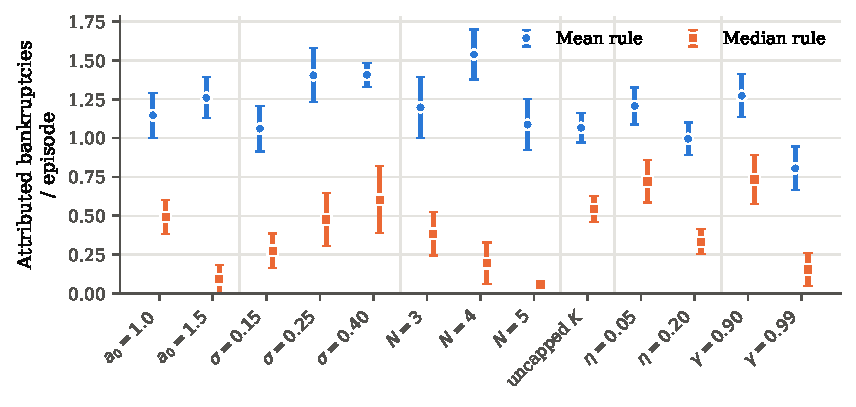
\includegraphics[width=0.95\linewidth]{figures/sensitivity.pdf}
\caption{All sellers learning, $3\times10^8$ steps, 10 seeds per point: attributed bankruptcies per episode under the mean and median rules when one feature of the market or of learning is changed. The $\sigma$ and $N$ axes use $\Phi=0.04$, $K_0=0.12$ so that every point is viable; $N$ uses a 7-price grid. Error bars: one standard error.}
\label{fig:sensitivity}
\end{figure}

\paragraph{Robustness.} We varied one feature at a time: the threshold $\delta$, the grid size $M$ and the audit budget $B$ (8 settings), and the outside option $a_0$, the price sensitivity $\sigma$, the number of sellers $N\in\{3,4,5\}$, uncapped capital, the learning rate $\eta$ and the discount $\gamma$ (13 settings; Figure~\ref{fig:sensitivity}). The mean rule produces more attributed bankruptcies than the median in all 21 settings, by $0.49$--$1.62$ per episode; the difference is significant after Holm's correction in 19 of them, and $p_{\mathrm{H}}=0.066$ in the other two ($\eta=0.05$, $\gamma=0.90$). Framing survives a real outside option ($a_0=1.5$: $1.26$ under the mean rule against $0.09$), uncapped capital ($1.07$ against $0.54$), and five sellers ($1.09$ against $0.06$). With four sellers and $\Nmin=3$, where the median never compares fewer than three prices, the mean rule causes $0.55$ attributed bankruptcies per episode against $0.18$ ($p_{\mathrm{H}}=0.026$).

\subsection{Framing does not need a lethal ban (H2)}
\label{sec:phase}

\begin{figure}[t]
\centering
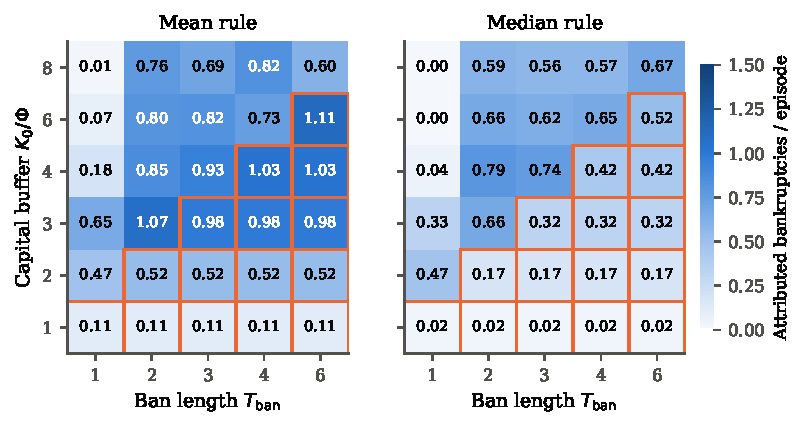
\includegraphics[width=0.92\linewidth]{figures/phase_diagram.pdf}
\caption{Phase diagram: attributed bankruptcies per episode with all sellers learning ($3\times10^8$ steps, 10 seeds per cell) as the capital buffer $K_0/\Phi$ and the ban length $\Tban$ vary. Outlined cells are those where one ban is lethal ($K_0\le\Tban\Phi$), the only region where H2 predicted framing.}
\label{fig:phase}
\end{figure}

H2 predicted framing only where one ban exhausts the victim's buffer. Figure~\ref{fig:phase} rejects it. Under the mean rule, the 15 cells where a banned rival survives average $0.63$ attributed bankruptcies per episode, as many as the lethal cells ($0.58$); in every cell with bans of at least two periods and $K_0\ge2\Phi$, framing is at least $0.52$. What stops framing is very short bans combined with a large buffer ($\Tban=1$, $K_0\ge4\Phi$: at most $0.18$). The mean rule is at least as exploitable as the median in 29 of the 30 cells. Training length matters here too: at $10^7$ steps the non-lethal cells average only $0.09$ against $0.39$ for the lethal ones, a pattern that would have appeared to confirm H2.

\paragraph{A transient of learning.} At $10^7$ steps, an all-learner market under a price cap of 0.60 with $\Nmin=2$ loses two firms per episode although no ban is attributable to a rival: step-level traces show sellers pricing above the cap, two being banned into bankruptcy, and the last one pricing at 1.50 once audits stop. At $3\times10^8$ steps this disappears: all three firms survive in every seed and prices settle at the cap ($0.59$). The ``race to be the last unregulated seller'' is a phase of learning, not a stable outcome.

\subsection{Behavioural traits (H3)}
\label{sec:traits}
\begin{figure}[t]
\centering
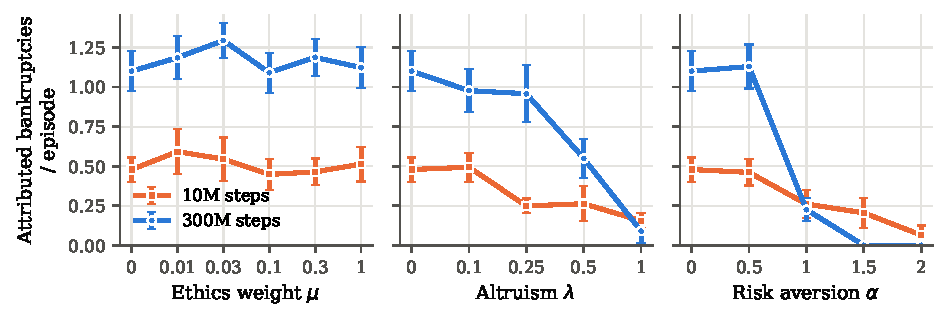
\includegraphics[width=0.95\linewidth]{figures/traits.pdf}
\caption{Attributed bankruptcies per episode as one trait is varied (all three sellers share the value; mean rule, $\delta=0.10$), at $10^7$ and $3\times10^8$ training steps. Ten seeds per point; error bars: one standard error.}
\label{fig:traits}
\end{figure}

We varied one trait at a time for all three learners, at $10^7$ and $3\times10^8$ steps (Figure~\ref{fig:traits}). \emph{Risk aversion} has the strongest effect: at $3\times10^8$ steps attributed bankruptcies fall from $1.10\se{0.13}$ at $\alpha=0$ to $0.23\se{0.07}$ at $\alpha=1$ and exactly zero at $\alpha\ge1.5$, where no seller is ever banned and all three survive in every seed (Spearman $\rho=-0.84$, $p_{\mathrm{H}}=0.004$). Framing is a gamble on a lethal audit; concave utility makes it unattractive. \emph{Altruism} also reduces framing, from $1.10$ to $0.09\se{0.08}$ at $\lambda=1$ ($\rho=-0.61$, $p_{\mathrm{H}}=0.004$); at $10^7$ steps this effect was weak and non-monotonic. The \emph{ethics} penalty has no detectable effect at either length ($1.09$--$1.30$ for every $\mu\in[0,1]$; $\rho=0.02$, $p_{\mathrm{H}}=0.90$). A likely reason is scale: at $\mu=1$ the penalty for one framed ban equals about ten periods of Nash profit, while eliminating both rivals raises per-period profit from $0.10$ to about $1.3$ over a discounted horizon of $1/(1-\gamma)=20$ periods, a gain of roughly 24 reward units against a penalty of at most 2.

\subsection{Further rules, audit selection, ban length, observation and trait mixtures}
\label{sec:more}

These studies complete the proposal's sweep (rule $\in$ \{mean, median, cap, z-score\}, $\Tban\in\{1,3,5,10\}$, trait mixtures), its baselines (omniscient planner; homogeneous all-ethical vs.\ all-predatory populations), its top-score-first audit variant, and its ban-timer observation ablation. All use the main-study protocol and seeds (\texttt{experiments/run\_promises.py}); a separate family of 28 comparisons with bootstrap intervals and Holm's correction is in \texttt{results/stats/promises\_comparisons.csv}.

\begin{table}[t]
\centering
\caption{Rules under uniform and top-score-first audits. Single learner vs.\ two Nash rivals (rivals bankrupted per episode, $2\times10^6$ steps, 20 seeds; identical under both audits except the learner's profit) and all three sellers learning ($3\times10^8$ steps, 10 seeds): attributed bankruptcies per episode, mean price, survivors, and welfare loss. Nash price 0.30.}
\label{tab:rules}
\small
\begin{tabular}{@{}lccccccc@{}}
\toprule
& Single & \multicolumn{4}{c}{All learners, uniform audit} & \multicolumn{2}{c}{Top-score audit} \\
\cmidrule(lr){2-2}\cmidrule(lr){3-6}\cmidrule(lr){7-8}
Rule & rivals bankr. & bankr. & price & survivors & SWL & bankr. & price \\
\midrule
Mean & 2.00 & 1.25 & 1.32 & 1.01 & 0.17 & 0.20 & 0.19 \\
Median & 0.00 & 0.41 & 0.77 & 1.65 & 0.12 & 0.00 & 0.15 \\
Cap 0.60 & 0.00 & 0.00 & 0.60 & 3.00 & 0.00 & 0.00 & 0.55 \\
z-score $\tau{=}0.5$ & 2.00 & 1.05 & 1.22 & 1.19 & 0.16 & 0.00 & 0.15 \\
z-score $\tau{=}1.0$ & 0.00 & 0.15 & 0.52 & 2.26 & 0.04 & 1.00 & 0.58 \\
Planner & 0.00 & 0.00 & 0.30 & 3.00 & 0.00 & 0.00 & 0.28 \\
\bottomrule
\end{tabular}
\end{table}

\paragraph{z-score.} Proposition~\ref{prop:vuln}(v) predicts the single-learner column of Table~\ref{tab:rules}: at $\tau=0.5$ any undercut flags both rivals, and the learner bankrupts both in all 20 seeds, exactly as under the mean rule ($2.00$ vs.\ $0$ under the median, $p_{\mathrm H}=0.003$); at $\tau=1$ one undercutter cannot produce $Z>1$ and the learner prices at Nash. With all sellers learning, $\tau=0.5$ is statistically indistinguishable from the mean rule ($1.05$ vs.\ $1.25$, $p_{\mathrm H}=1.0$) and $\tau=1$ frames far less ($0.15$, $p_{\mathrm H}=0.003$). The proposal expected the z-score to be a weaker attack surface because crashing buys nothing beyond a small undercut; the opposite reading is the relevant one: a small undercut is all it takes, so a low threshold makes framing cheaper, not harder.

\paragraph{Omniscient planner.} Judging each price against the seller's own Nash price removes the lever entirely: with all sellers learning there are no bankruptcies, all three sellers survive in every seed, the mean price is exactly the Nash price and $\Delta=\mathrm{SWL}=0$ (mean rule: $1.25$ bankruptcies and $\mathrm{SWL}=0.17$; both differences $p_{\mathrm H}=0.003$). This is the proposal's upper bound on welfare recovery. It requires cost information the watchdog does not have; the cap enforced by escrow (Section~\ref{sec:defences}) comes close without it.

\paragraph{Top-score-first audits.} Against honest rivals, auditing the most suspicious seller first does not help: the single learner still bankrupts both rivals in every seed, and earns slightly more ($1.316$ vs.\ $1.311$), since the rival it frames is now audited with certainty. With all sellers learning the rule changes the game. Because the highest-priced seller is always audited, sellers race below Nash (mean price $0.15$--$0.19$ under the mean, median and $\tau=0.5$ rules, against a Nash price of $0.30$). Framing largely disappears (mean rule $1.25\to0.20$, $p_{\mathrm H}=0.014$, nine seeds of ten without it; median and $\tau=0.5$ to zero), but under the $\tau=1$ z-score it becomes systematic: two sellers undercut together and the third, now audited every period, is framed in every seed ($1.00$ vs.\ $0.15$, $p_{\mathrm H}=0.004$; Proposition~\ref{prop:vuln}(v) with $k=2$). Top-score auditing trades framing for a price war, and it makes coalition framing deterministic where the threshold permits it.

\paragraph{Ban length.} With $K_0=3\Phi$ a ban of $\Tban\ge3$ periods is lethal, and $\Tban=3,4,5,10$ give results identical to the last digit (mean rule $1.25$, median $0.41$): a banned seller is bankrupt after three periods, so a longer timer never runs out, and learners only observe that a rival is inactive. Once a ban kills, its length is irrelevant. One-period bans reduce framing under the mean rule to $0.35$ ($p_{\mathrm H}=0.003$) and leave the median rule at $0.28$ (vs.\ $0.41$, not significant).

\paragraph{Observing ban timers.} The proposal's ablation gives learners each seller's exact status (active, remaining ban $1,\dots,\Tban$, or bankrupt) instead of an inactive bit, enlarging the observation space from 31,944 to 862,488. A single learner then frames in 0 of 20 seeds at $2\times10^6$ steps (profit $0.35$), but in 20 of 20 seeds at $2\times10^7$ and $10^8$ steps, with the same profit as with the coarse observation ($1.310$ vs.\ $1.312$). With all sellers learning ($3\times10^8$ steps) framing is $0.80$ vs.\ $1.25$ under the mean rule and $0.37$ vs.\ $0.41$ under the median, neither significant after correction. The coarse observation hides nothing the attack needs; it only speeds up learning.

\paragraph{Trait mixtures.} Table~\ref{tab:mix} varies the composition of the population under the mean rule. Homogeneous risk-averse ($\alpha=2$) and altruistic ($\lambda=1$) populations do not frame ($0$ and $0.09$), but one risk-neutral or selfish seller among them restores framing to the all-neutral level ($1.24$ and $1.10$, both $p_{\mathrm H}=0.003$ against the homogeneous population). The protected sellers then frame as well: averse sellers cause $0.34$ bankruptcies each and altruistic sellers $0.25$, against $0.56$ and $0.59$ for the neutral or selfish seller in the same markets; these within-market differences are not significant after correction ($p_{\mathrm H}=0.45$ and $0.17$). The neutral or selfish seller is, if anything, also the more frequent victim ($0.73$ vs.\ $0.58$ and $0.66$ vs.\ $0.53$ bankruptcies per episode). The ethics penalty has no effect in any composition, as in the homogeneous sweep (all-ethical vs.\ all-predatory: $1.12$ vs.\ $1.10$, $p_{\mathrm H}=1.0$). Trait-based protection therefore requires that \emph{every} seller has the trait: once framing pays for someone, it spreads.

\begin{table}[t]
\centering
\caption{Trait mixtures, mean rule, all sellers learning ($3\times10^8$ steps, 10 seeds). Attributed bankruptcies per episode in total and caused by each seller type, and mean price. In each mixture the first type listed is the minority type when it is a single seller.}
\label{tab:mix}
\small
\begin{tabular}{@{}lcccc@{}}
\toprule
Population & total & by neutral/selfish & by trait seller (each) & price \\
\midrule
All neutral & 1.10 & 0.37 & --- & 1.39 \\
All risk-averse ($\alpha=2$) & 0.00 & --- & 0.00 & 0.15 \\
1 neutral + 2 averse & 1.24 & 0.56 & 0.34 & 1.26 \\
2 neutral + 1 averse & 1.26 & 0.44 & 0.37 & 1.35 \\
All altruistic ($\lambda=1$) & 0.09 & --- & 0.03 & 0.25 \\
1 selfish + 2 altruistic & 1.10 & 0.59 & 0.25 & 1.13 \\
2 selfish + 1 altruistic & 1.32 & 0.55 & 0.21 & 1.41 \\
All ethical ($\mu=1$) & 1.12 & --- & 0.37 & 1.26 \\
1 predator + 2 ethical & 1.33 & 0.55 & 0.39 & 1.29 \\
2 predators + 1 ethical & 1.07 & 0.39 & 0.28 & 1.15 \\
\bottomrule
\end{tabular}
\end{table}

\subsection{Defences against learners}
\label{sec:defences}

\begin{table}[t]
\centering
\caption{Defences. Rival bankruptcies per episode against a scripted \emph{patient} attacker that holds 0.15 while audits run (5 seeds), against a single Q-learner after $2\times10^6$ and $3\times10^8$ training steps (20 seeds; fixed Nash rivals), and total bankruptcies, survivors and mean price when all three sellers learn for $3\times10^8$ steps (10 seeds). Mean (standard error); $\delta=0.10$, lethal bans. The Nash price is 0.30.}
\label{tab:defences}
\small
\begin{tabular}{@{}lcccccc@{}}
\toprule
& Patient attacker & \multicolumn{2}{c}{Single learner} & \multicolumn{3}{c}{All learners, $3\times10^8$} \\
\cmidrule(lr){2-2}\cmidrule(lr){3-4}\cmidrule(lr){5-7}
Rule & rival exits & $2\times10^6$ & $3\times10^8$ & bankruptcies & survivors & mean price \\
\midrule
Mean            & 2.00\se{0.00} & 2.00\se{0.00} & 2.00\se{0.00} & 2.08\se{0.02} & 0.92\se{0.02} & 1.44 \\
Median          & ---           & ---           & ---           & 1.72\se{0.16} & 1.28\se{0.16} & 1.04 \\
EMA $\beta{=}0.80$ & 2.00\se{0.00} & 0.00\se{0.00} & 2.00\se{0.00} & 0.72\se{0.29} & 2.28\se{0.29} & 0.50 \\
EMA $\beta{=}0.95$ & 2.00\se{0.00} & 0.00\se{0.00} & 0.00\se{0.00} & 1.00\se{0.33} & 2.00\se{0.33} & 0.63 \\
EMA $\beta{=}0.99$ & 2.00\se{0.00} & 0.00\se{0.00} & 0.00\se{0.00} & ---           & ---           & ---  \\
Mean + escrow   & 0.00\se{0.00} & 0.00\se{0.00} & 0.00\se{0.00} & 0.00\se{0.00} & 3.00\se{0.00} & 0.69 \\
Cap 0.60 + escrow & ---         & 0.00\se{0.00} & ---           & 0.00\se{0.00} & 3.00\se{0.00} & 0.59 \\
\bottomrule
\end{tabular}
\end{table}

We tested both defences of Proposition~\ref{prop:def} against learners, and escrow combined with a price cap (Table~\ref{tab:defences}).

\emph{EMA delays framing but does not prevent it.} A scripted attacker that simply holds 0.15 bankrupts both rivals in every episode for every $\beta$ we tried, as Proposition~\ref{prop:def}(i) predicts. Learners find this more slowly: after $2\times10^6$ steps no single learner frames under any EMA rule, but after $3\times10^8$ steps it frames both rivals in all 20 seeds at $\beta=0.80$, where the attack needs 4 periods; at $\beta\ge0.95$, where it needs 16 or more, none did. With all sellers learning, EMA reduces bankruptcies from 2.08 to 0.72--1.00 per episode ($p_{\mathrm{H}}\le0.011$), but outcomes split across seeds, and the replay test (Table~\ref{tab:replay}) shows that most of the remaining exits are framing: the one-period metric attributes only 15--23\% of bans to rivals, the replay 45--49\%, and $0.64$ bankruptcies per episode at $\beta=0.95$ would not have happened had the rivals stayed honest. EMA protects only to the extent that learners fail to find a slower attack.

\emph{Escrow removes framing entirely.} No seller is ever suspended, no sanction is attributed to a rival in any setting, as Proposition~\ref{prop:def}(ii) predicts, and all three sellers survive in every seed. The cost is weak price discipline: with all sellers learning, prices settle at 0.54--0.85 (mean 0.69), well above the Nash price of 0.30 and close to an unregulated market (0.68 at $3\times10^8$ steps).

\emph{A cap enforced by escrow removes framing and keeps prices down.} A cap judges each seller on its own price, so no rival can trigger it (Proposition~\ref{prop:vuln}(iv)); escrow removes the lethal ban. Together, with all sellers learning, no seller is ever sanctioned or bankrupted, all three survive in every seed, and prices settle at the cap ($0.59$, against $0.69$ under mean + escrow); a single learner prices at Nash in all 20 seeds. Once learning has converged, a cap enforced by suspensions behaves the same way (Section~\ref{sec:phase}), but without suspensions there is no lethal sanction to gamble on, so the learning-phase ``race to the last seller'' cannot arise at all. Prices are held at the cap, not at Nash: how much this protects consumers depends on where the cap is set, and learners settle just below it (collusion index $0.25$).

\paragraph{Welfare.} The collusion index $\Delta=(\bar\pi-\pi^N)/(\pi^M-\pi^N)$ and the social welfare loss $\mathrm{SWL}$ (total surplus relative to Nash) summarise the damage. When the single learner frames its rivals, $\Delta=0.89$ and $\mathrm{SWL}=0.18$. With all sellers learning ($3\times10^8$ steps), $\mathrm{SWL}$ is $0.18$ under the mean rule, $0.15$ under the median, $0.06$--$0.08$ under EMA, and $0.005$ under mean + escrow; a price cap loses nothing whether enforced by suspensions ($0.000$) or by escrow ($0.001$). With almost no outside option, escrow's higher prices mostly move surplus from consumers to sellers rather than destroying it.

%% ===================================================================
\section{Discussion and Limitations}
\label{sec:discussion}

\begin{table}[t]
\centering
\caption{Hypotheses from the proposal and what we found.}
\label{tab:scorecard}
\small
\begin{tabularx}{\linewidth}{@{}lXl@{}}
\toprule
& Finding & Verdict \\
\midrule
H1 & One learner frames under the mean rule in every seed and never under the median or the cap; with all learners the mean rule is more exploitable in all 21 variations, but the median is not immune once two firms remain. & Supported, with a caveat \\
H2 & Framing is as frequent where a banned rival survives as where one ban kills; only one-period bans with large buffers stop it. & Rejected \\
H3 & Risk aversion and altruism sharply reduce framing; risk aversion $\alpha\ge1.5$ removes it. An ethics penalty up to $\mu=1$ has no effect. & Partly supported \\
H4 & Learners reach the exact optimum when one ban suffices and fall short as the attack needs more repeated bans. & Supported \\
New & Two deep learners frame honest sellers together, then each other; the median rule stops this while they are a minority. & --- \\
New & EMA delays framing; escrow alone removes it but weakens price discipline; a cap enforced by escrow removes it and holds prices at the cap. & --- \\
\bottomrule
\end{tabularx}
\end{table}

Table~\ref{tab:scorecard} summarises the hypotheses. A regulator whose benchmark is computed from the prices it judges gives every seller a lever over its rivals' treatment, and independent learners find that lever without being told about it, reaching the exact optimum when the attack is short. A median benchmark removes the lever for a lone undercutter but only while enough sellers remain; a cap removes it entirely. Smoothing the benchmark over time only slows the attack down, and learners can wait. Replacing suspensions with fines on excess profit takes away the reward for framing altogether, because a framed seller has no excess profit to lose, but on its own it is too weak to keep prices down; applied to a fixed price cap, it gives a rule that no seller can turn against a rival and that still holds prices down. When several algorithmic sellers are present, they need not coordinate explicitly: independent learners discover a joint attack on honest sellers and then compete for the monopoly it creates. Across all of these results, short training repeatedly gave the wrong picture: it understated framing, made H2 look true, and produced a ``race to the last seller'' that vanishes at convergence.

\paragraph{Limitations.} The market is synthetic and is not calibrated to a platform, although the main comparison survives a real outside option, uncapped capital and changes to demand and learning parameters. Tabular learners limit the all-learning studies to $N\le5$ (at $N=6$ each learner would need about $2\times10^7$ observations even with 7 prices); deep Q-networks reach $N=10$, but we have run at most two deep learners at once, not a market in which every seller is a deep learner, where the tabular results needed $3\times10^8$ steps. Observations are not Markov and learners are independent, so frozen policies are not equilibria \citep{busoniu2008}; the exact benchmark covers only one learner against fixed rivals, and only cells where a ban is lethal or nearly so. The replay test holds a rival at Nash and lets everyone else follow their frozen policies; with reactive learners, longer windows need not attribute more. We use 10--20 seeds per condition, report bootstrap intervals and Holm-corrected permutation tests for key comparisons, and did not preregister the studies.

\paragraph{Future work.} (i) Markets in which every seller is a deep learner, and more learners in larger markets; this needs a vectorised GPU simulator to reach the required training length, which we have implemented and validated against the simulator used here. (ii) An exact or approximate best response when rivals survive bans, for example by porting the solver to C++, and an exact analysis of the EMA rule. (iii) Honest sellers that defend themselves, by following prices down or by jointly retaliating against an attacker. (iv) Rerunning the proposal's extensions (a learning regulator, a demand shock) on the corrected engine. (v) Mixed populations of traits, and an ethics penalty scaled to the monopoly gain.

%% ===================================================================
\section{Conclusion}
A relative-price watchdog can be turned against the sellers it is meant to discipline. A single learning seller, tabular or deep, discovers that cutting its price to get honest rivals suspended is the optimal route to monopoly under a mean rule, in markets of up to ten sellers. Two learners frame honest sellers together and then each other, and fully learning markets frame each other too, causally and robustly, under the mean rule more than the median. Framing does not require a lethal ban. Smoothing the benchmark only delays the attack. A price cap enforced by fines on excess profit, rather than suspensions, gives no seller a lever over its rivals and still holds prices down. Designers of automated market supervision should prefer references and penalties that a seller cannot turn against its rivals, and should evaluate them against learners trained long enough to find the slow attacks.

\paragraph{Code and reproducibility.} All code, result CSVs, and figure scripts are at \url{https://github.com/hemtilva/WeaponzingWatchdog}. Every table and figure here is produced by a script listed in the repository README.

%% ===================================================================
\section*{Contributions}

\begin{table}[h]
\centering
\small
\begin{tabularx}{\linewidth}{@{}lXXl@{}}
\toprule
Member & Assigned in proposal & Delivered & Fulfilled? \\
\midrule
Satvik Sharma & Market engine, exact best-response baseline, Extension B & \textit{[to be completed]} & \textit{[yes/partly/no]} \\
Krish Goradia & Q-learning agents with traits, harm attribution and metrics, DQN ablation & \textit{[to be completed]} & \textit{[yes/partly/no]} \\
Hem Tilva & Sweep orchestration, analysis and plots, Extension A & \textit{[to be completed]} & \textit{[yes/partly/no]} \\
\bottomrule
\end{tabularx}
\end{table}

\bibliographystyle{unsrtnat}
\bibliography{references}

\end{document}
